\documentclass{article}
\usepackage[utf8]{inputenc}
\usepackage{amsmath}
\usepackage[french]{babel}
\usepackage[a4paper, margin=1in]{geometry}
\usepackage[default]{raleway}
\usepackage{graphicx}
\usepackage{listings}
\usepackage{xcolor}
\usepackage{amssymb}
\usepackage{algorithm}
\usepackage{algorithmic}

% Paramètres d'affichage du code
\lstset{
    basicstyle=\ttfamily\footnotesize,
    backgroundcolor=\color{gray!10},
    frame=single,
    breaklines=true,
    keywordstyle=\color{blue}\bfseries,
    commentstyle=\color{green!60!black},
    stringstyle=\color{red!70!black},
    numbers=left,
    numberstyle=\tiny\color{gray},
    stepnumber=1,
    numbersep=10pt,
    showspaces=false,
    showstringspaces=false,
    tabsize=4,
    captionpos=b
}

\begin{document}

% Page de titre
\begin{titlepage}
    \centering
    \vspace*{1cm}
    \Huge
    \textbf{Compte-Rendu : Simulation de Contrôle Robotique}
    \vspace{1.5cm}
    \LARGE \\
    \textbf{Paul TESSON}
    \vspace{0.5cm}
    \large \\
    \textbf{Numéro étudiant :} 20210145
    \vfill
    
\includegraphics[width=0.5\textwidth]{Logo_ENIB_2012.png}
    \vfill
    \Large
    \textbf{\today}
\end{titlepage}

\tableofcontents
\newpage
\section{Objectifs}
Ce projet vise à implémenter et analyser un système de contrôle robotique en utilisant une approche basée sur des réseaux de neurones. Les principaux objectifs incluent :
\begin{itemize}
    \item Le développement d'une simulation pour contrôler un robot mobile (Pioneer) vers une cible donnée.
    \item L'entraînement du réseau de neurones pour optimiser les commandes du robot.
    \item L'analyse des erreurs de position et d'orientation pour évaluer les performances.
    \item La visualisation graphique des erreurs pour identifier les zones d'amélioration.
\end{itemize}

\section{Description de la Simulation}
La simulation repose sur un robot Pioneer simulé dans un environnement virtuel (Coppeliasim). Le robot utilise des commandes issues d'un réseau de neurones (NN) pour ajuster sa position et son orientation en fonction d'une cible (0 0 0).

\subsection*{Configuration Initiale}
Le système inclut :
\begin{itemize}
    \item Un robot Pioneer simulé par \texttt{VrepPioneerSimulation}.
    \item Un réseau de neurones comprenant une couche cachée de 30 neurones.
    \item Des poids initialisés (aléatoirement) avec possibilité de chargement d'un réseau précédemment entraîné.
    \item l'apprentissage est non supervisé : il n'y a pas de séries d'exemples
\end{itemize}

\section{Approche de Contrôle}
\subsection*{Calcul des Erreurs}
Les erreurs en position $x$, $y$ et orientation $\theta$ sont calculées comme suit :
\begin{align*}
    e_x &= (x_{\text{actuel}} - x_{\text{cible}}) \cdot \alpha_x \\
    e_y &= (y_{\text{actuel}} - y_{\text{cible}}) \cdot \alpha_y \\
    e_\theta &= \left(\theta_{\text{actuel}} - \theta_{\text{cible}} - \theta_s(x, y)\right) \cdot \alpha_\theta
\end{align*}
avec $\theta_s(x, y)$ déterminant une correction d'orientation en fonction de la position.

\subsection*{Optimisation}
Le réseau de neurones ajuste les commandes de vitesse des roues basées sur les erreurs normalisées. Un algorithme de propagation par gradient est utilisé pour minimiser un critère quadratique d'erreur.

\newpage
\section{Modifications du Code Python}
Pour améliorer le projet, plusieurs modifications ont été apportées au code Python. Ces changements incluent l'ajout de fonctionnalités pour la visualisation des erreurs et de la trajectoire du robot, ainsi que l'augmentation du nombre de neurones dans la couche cachée du réseau de neurones. Les détails de ces modifications sont les suivants :

\subsection*{Ajout de la Visualisation Graphique}
Des fonctions ont été intégrées pour tracer les erreurs enregistrées et la trajectoire du robot. Ces tracés permettent de mieux comprendre les performances du système en termes d'erreurs de position et d'orientation. Voici un aperçu des changements (voir listenning ~\ref{listing:plotFunc}):
\begin{itemize}
    \item Ajout de la méthode \texttt{plot\_errors()} pour afficher les erreurs en $x$, $y$ et $\theta$ à chaque étape de l'entraînement.
    \item Ajout de la méthode \texttt{plot\_trajectory()} pour tracer la trajectoire suivie par le robot.
\end{itemize}

\subsection*{Récupération des Valeurs pour les Tracés}
Le code a été modifié pour stocker les valeurs des erreurs et les positions à chaque étape. Ces valeurs sont ensuite utilisées pour créer les graphiques.

\subsection*{Modification de la Structure du Réseau de Neurones}
Le nombre de neurones dans la couche cachée du réseau a été augmenté de 30 à 40. Cette modification vise à améliorer la capacité de prise de décision de notre robot . Il faut par contre plus de temps pour qu'il apprenne correctement dans une situation bien définie ( c'est pour cette raison que nous n'avons pas mis plus de neurones). Si notre apprentissage est bien fait, alors le robot aura de meilleures performances (voir Listing~\ref{listing:variables}).

\subsection*{Extrait du Code Modifié}
\begin{lstlisting}[language=Python, caption=Extract of plot functions in online\_trainer.py, label=listing:plotFunc]
def plot_errors(self):
    """Plot the recorded errors."""
    plt.figure(figsize=(12, 6))

    # Subplot for X errors
    plt.subplot(3, 1, 1)
    plt.plot(self.errors_x, label='X Error', color='blue', linewidth=1.5)
    plt.xlabel('Iterations')
    plt.ylabel('X Error')
    plt.title('X Error')
    plt.legend()
    plt.grid(True)
    plt.xticks(rotation=45)

    # Subplot for Y errors
    plt.subplot(3, 1, 2)
    plt.plot(self.errors_y, label='Y Error', color='green', linewidth=1.5)
    plt.xlabel('Iterations')
    plt.ylabel('Y Error')
    plt.title('Y Error')
    plt.legend()
    plt.grid(True)
    plt.xticks(rotation=45)

    # Subplot for Theta errors
    plt.subplot(3, 1, 3)
    plt.plot(self.errors_theta, label='Theta Error', color='red', linewidth=1.5)
    plt.xlabel('Iterations')
    plt.ylabel('Theta Error')
    plt.title('Theta Error')
    plt.legend()
    plt.grid(True)
    plt.xticks(rotation=45)

    plt.tight_layout()
    plt.show()

def plot_trajectory(self):
    """Plot the robot's trajectory."""
    x_values = [pos[0] for pos in self.positions]
    y_values = [pos[1] for pos in self.positions]

    plt.figure(figsize=(10, 10))
    plt.plot(x_values, y_values, marker='o', linestyle='-', color='b', label='Trajectory')
    plt.title('Robot Trajectory')
    plt.xlabel('X Position')
    plt.ylabel('Y Position')
    plt.axhline(0, color='black', linewidth=1)  # X-axis
    plt.axvline(0, color='black', linewidth=1)  # Y-axis
    plt.grid(True)
    plt.legend()
    plt.show()
\end{lstlisting}
\begin{lstlisting}[language=Python, caption=Extract of variables in run.py, label=listing:variables]
# Initialize the robot and the neural network
robot = VrepPioneerSimulation()
HL_size = 30  # Number of neurons in the hidden layer
network = NN(3, HL_size, 2)
\end{lstlisting}

\section{Visualisation de la trajectoire du robot}
La figure ci-dessus nous montre la trajectoire du robot 
\section{Visualisation des Erreurs}
Les erreurs enregistrées pour $x$, $y$, et $\theta$ sont affichées graphiquement pour évaluer les performances. Ces graphiques permettent d'identifier les schémas d'erreurs et les améliorations potentielles.

\begin{figure}[ht!]
    \centering
    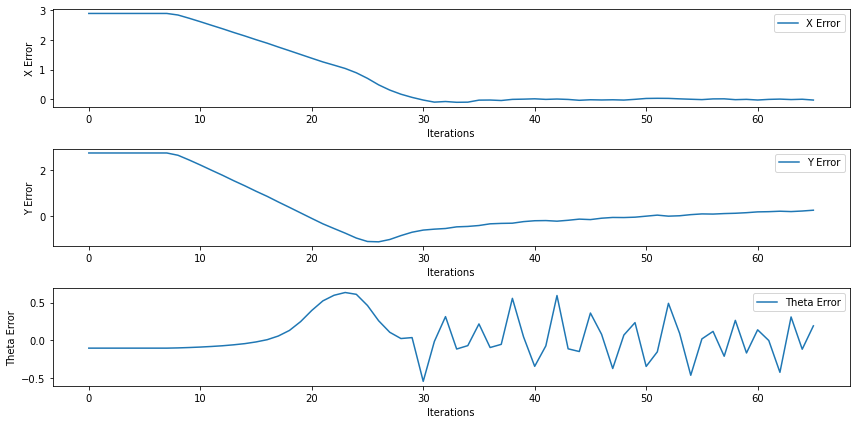
\includegraphics[width=1\textwidth]{errors_plot.png} % Remplacer par le chemin vers le graphique généré
    \caption{Graphique des erreurs en position ($x$, $y$) et orientation ($\theta$).}
    \label{fig:errors}
\end{figure}

\newpage
\section{Limites et Améliorations}
\subsection*{Limites}
\begin{itemize}
    \item Les ajustements peuvent être trop sensibles à des perturbations locales.
    \item Le robot 
    \item L'absence d'un facteur d'inertie entraîne des oscillations dans les commandes.
\end{itemize}

\subsection*{Améliorations Proposées}
\begin{itemize}
    \item Introduire un filtre pour lisser les commandes du réseau de neurones.
    \item Augmenter la complexité du réseau avec plus de neurones ou des couches additionnelles.
    \item Incorporer des méthodes d'apprentissage adaptatif pour optimiser les poids plus rapidement.
\end{itemize}

\section{Conclusion}
Ce projet a permis de simuler avec succès un robot mobile contrôlé par un réseau de neurones. La visualisation des erreurs a offert une vue précieuse sur les performances du système et les possibilités d'amélioration. Les prochaines étapes incluent l'ajout de fonctions de lissage et l'exploration de configurations de réseaux plus complexes.

\newpage
\appendix
\section{Annexe : Code Source Complet}

\lstinputlisting[
  language=Python, 
  caption= run.py, 
  label=code:run
]{run.py}

\lstinputlisting[
  language=Python, 
  caption= online\_trainer.py, 
  label=code:onlineTrainer
]{online_trainer.py}




La stratégie pour éviter un minimum local est définie comme suit :

\[
\theta_s =
\begin{cases} 
\arctan(10 \cdot Y_M(t)), & \text{si } X_M(t) \geq 0, \\[10pt]
\arctan(-10 \cdot Y_M(t)), & \text{si } X_M(t) \leq 0.
\end{cases}
\]

Donc il faut implémenter ce code 

\begin{lstlisting}[language=Python, caption=Résolution du problème de propagation du gradient, label=listing:grad]
def theta_s(x,y):
if x>=0:
    return 1*math.atan(1*y)
    #return (math.pi)/4*2*x*math.exp(-x*x)

if x<=0:
    return 1*math.atan(-1*y)
    #return -(math.pi)/4*2*x*math.exp(-x*x)
\end{lstlisting}


\end{document}

